\newcommand\titelpage{%
\begin{tikzpicture}[overlay, remember picture]
    % green bar
    \fill[cvgreen] (current page.north west) rectangle ([xshift=5cm]current page.south west);
    % gray bar
    \fill[cvgray] ([yshift=-5cm]current page.north west) rectangle ([yshift=-10cm]current page.north east);
    % title and date
    \node[cvtext,right] at ([yshift=-7cm]current page.north west) {\Huge\bfseries Mathe-Notizen f"ur Selbstudium};
    \node[cvtext,right] at ([yshift=-8cm]current page.north west) {\Huge 1. Auflage};
    \node[cvtext,above left] at ([xshift=-1cm,yshift=-9.5cm]current page.north east) {\Huge\bfseries vom \today };
    % cover photo
    \node[inner sep=0pt,below right] (image) at ([xshift=5cm,yshift=-10cm]current page.north west)
    {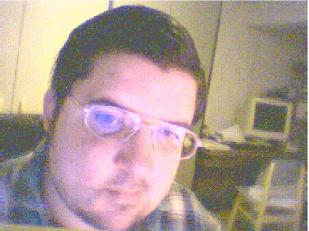
\includegraphics[width=11cm,height=9cm]{pics/me.jpg}};
    % name and address
    \node[fill=white,drop shadow,align=center,text width=6.4cm,inner sep=0.3cm,below] (name) at (image.south)
        {\LARGE Jens Kallup};
    \node[text width=15cm,inner sep=0.3cm,below right] at (name.south west) {\Large\obeylines%
        Langensalzer Str. 30\\
        99817 Eisenach\\
        Tel.: 03691 / \\
        E-Mail: jkallup@web.de
    };
    % attachments
    \node[black,text width=5cm,inner sep=0.3cm,above right] at ([yshift=1cm]current page.south west) {\large\obeylines%
        \textbf{Inhalt:}\\[4pt]
        Eigene Gedanken zu:\\[3pt]
        de.sci.mathematik \\
        de.sci.informatik
    };
\end{tikzpicture}}

